\documentclass{article}
\usepackage{graphicx}
\begin{document}
\usepackage{graphicx}
\begin{center}
    {\Huge be nam khoda} \\[1cm]
    {\LARGE projeye kargah} \\[0.5cm]
    {\large Mohammad Matin Roozbehani} \\[0.5cm]
    {\large 402531387} \\[1cm]
    \rule{\linewidth}{0.4mm}
\end{center}

\vspace{1cm}

\section*{fehrest mataleb}
\begin{itemize}
    \item taklif: inja mitavanid tozihat marboot be taklif ra ezafe konid.
\end{itemize}

\newpage

\section*{taklif}
\textbf{1.1 Repository Initialization and Commits}

\section*{list mataleb}
\textbf{1.1 Repository Initialization and Commits}

\section{Git and GitHub}
\subsection{Repository Initialization and Commits}
\subsection{GitHub Actions for LaTeX Compilation}

\section{Exploration Tasks}
\subsection{Vim Advanced Features}
\subsection{Memory Profiling}
\subsubsection{Memory Leak}
\subsubsection{Memory Profilers}
\subsection{GNU/Linux Bash Scripting}
\subsubsection{fzf}
\subsubsection{Using fzf to Find Your Favorite PDF}
\subsubsection{Opening the File Using Zathura}

\section{Git and FOSS}
\subsection{README.md}
\subsection{Issues}
\subsection{FOSS Contribution}










\section*{taklif}

\textbf{1.1 Repository Initialization and Commits}

\textbf{Setting Up the Repository} \\
To set up the repository, I first went to GitHub and created a new repository named Final-Assignment. During the repository creation, I disabled the Initialize this repository with a README option. After creating the repository, I used the git clone command to clone it to my local system.

\begin{verbatim}
git clone https://github.com/username/Final-Assignment.git
cd Final-Assignment
\end{verbatim}

\textbf{Creating the LaTeX File and Making the First Commit} \\
Inside the local repository, I created a new file called assignment.tex and added initial content. I then added the changes to the staging area using git add and committed them with git commit. Finally, I pushed the changes to the GitHub repository.

\begin{verbatim}
git add assignment.tex
git commit -m "Add initial LaTeX file"
git push origin main
\end{verbatim}

\textbf{Setting Up Directory Structure and Additional Files} \\
To better organize the project, I created directories for sections and images and placed some LaTeX files like introduction.tex and git.tex in the sections directory.

\begin{verbatim}
mkdir sections images
touch sections/introduction.tex sections/git.tex
\end{verbatim}

\textbf{Making Regular Commits} \\
After each modification, I tracked and committed the changes using git add and git commit, and then pushed them to GitHub.

\begin{verbatim}
git add sections/git.tex
git commit -m "Added Git section to LaTeX document"
git push origin main
\end{verbatim}

\textbf{Using Tags to Trigger GitHub Actions} \\
To trigger GitHub Actions for automatic LaTeX PDF compilation, I used tags. I created a new tag and pushed it to GitHub.

\begin{verbatim}
git tag v1.0
git push origin v1.0
\end{verbatim}















\section*{1.2 GitHub Actions for LaTeX Compilation}

\textbf{Steps to Set Up GitHub Actions for Automatic LaTeX Compilation}

To set up GitHub Actions for automatic LaTeX compilation, I followed these steps:

1. First, I created a folder named `.github/workflows` in my GitHub repository.
2. Then, I created a YAML file named `latex.yml` inside this folder to define the GitHub Actions configuration.
3. Inside the `latex.yml` file, I added the following configuration to automatically compile the LaTeX file:

\begin{verbatim}
name: Build LaTeX PDF

on:
  push:
    branches:
      - main
  tags:
    - 'v*'

jobs:
  build:
    runs-on: ubuntu-latest

    steps:
      - name: Checkout repository
        uses: actions/checkout@v2

      - name: Set up TeX Live
        uses: yml2latex/texlive-action@v1
        with:
          texlive-version: "2020"

      - name: Compile LaTeX file
        run: |
          pdflatex -interaction=nonstopmode assignment.tex
          pdflatex -interaction=nonstopmode assignment.tex
      - name: Upload PDF as artifact
        uses: actions/upload-artifact@v2
        with:
          name: assignment-pdf
          path: assignment.pdf
\end{verbatim}

4. After setting up the YAML file, every time I add a new tag to the repository, GitHub Actions automatically runs the LaTeX compilation process and provides the resulting PDF in the "Artifacts" section.

\textbf{Challenges}

- The first challenge I encountered was ensuring the proper installation of the correct version of TeX Live, which required some additional setup.
- Sometimes, errors occurred during the LaTeX file compilation due to missing packages or incorrect settings, requiring further investigation.
- Additionally, after each modification to the LaTeX file, I needed to ensure that the PDF was regenerated properly and that the process ran smoothly without issues.









\section*{Advanced Vim Features}

Here are three advanced and lesser-known Vim features that may not have been covered in class:

\subsection*{1. Vim Sessions (Saving and Restoring State)}
One interesting feature of Vim is the ability to use Sessions, which allows you to save the current state and open files, then restore them at a later time. This is particularly useful when working on large projects or multiple files and you don't want to manually reopen them each time.

To save a session, you can use the following command:
\begin{verbatim}
:mksession! ~/my_session.vim
\end{verbatim}

To restore the session and bring back the previous state:
\begin{verbatim}
vim -S ~/my_session.vim
\end{verbatim}

This method ensures that you can return to exactly where you left off, with the files and settings as they were.

\subsection*{2. Vim Marks (Bookmarking Points)}
Marking different points in your files can be very helpful for quick editing or navigation in long files. With Marks, you can save locations you need and return to them later.

To mark a location, simply use the \texttt{m} command followed by a letter:
\begin{verbatim}
ma
\end{verbatim}
This saves a mark named \texttt{a} at the current position.

To go to a marked point:
\begin{verbatim}
'a
\end{verbatim}
This command takes you to the point marked with \texttt{a}.

This feature is extremely useful for quickly navigating between different parts of a file.

\subsection*{3. Macros in Vim (Automating Tasks)}
Macros in Vim allow you to record a series of commands and play them back automatically. This feature is very helpful for repetitive tasks.

To start recording a macro, use the \texttt{q} command followed by a letter:
\begin{verbatim}
qa
\end{verbatim}
This starts recording a macro named \texttt{a}.

Then, type the commands you want to record.

To stop recording, press \texttt{q} again:
\begin{verbatim}
q
\end{verbatim}

To execute the macro, just type the corresponding letter:
\begin{verbatim}
@a
\end{verbatim}

This feature is extremely useful when you have many repetitive tasks and can save a lot of time.










\section*{Memory Analysis}

\subsection*{2.2.1 Memory Leak}
Memory leak refers to a situation where memory requested by a program is not freed after it is no longer needed. As a result, the memory remains allocated and may cause a decrease in performance or crash the program. Memory leaks occur when memory is not properly released using functions like \texttt{free()} in C.

In C, when you allocate memory using functions such as \texttt{malloc()} or \texttt{calloc()}, you must free that memory after use using \texttt{free()}. Otherwise, the allocated memory becomes inaccessible but still belongs to the system.

Example:
\begin{verbatim}
int* ptr = malloc(sizeof(int)); // memory allocation
*ptr = 5; // using the memory
// forgetting to free the memory
\end{verbatim}
In the example above, the memory allocated for the pointer \texttt{ptr} is not freed, resulting in a memory leak.

\subsection*{2.2.2 Memory Profilers}
To identify and fix memory leaks, memory profiling tools such as \textbf{Valgrind} come in handy. \textbf{Valgrind} is a powerful tool for analyzing programs and can detect memory leaks, unauthorized memory usage, and similar issues.

To use Valgrind to check for memory leaks, you simply run your program with this tool. For example:
\begin{verbatim}
valgrind --leak-check=full ./my_program
\end{verbatim}
The \texttt{--leak-check=full} option causes Valgrind to check for all memory leaks and report the locations where leaks occurred.

This tool is especially useful during development and debugging, as it helps prevent long-term memory issues that can affect program performance.






\subsection*{2.2.1 Memory Leak}
\textbf{English:} 
Memory leak occurs when a program allocates memory dynamically (e.g., using \texttt{malloc()} or \texttt{calloc()}) but fails to release it when it's no longer needed. This causes the memory to remain occupied, even though it is no longer accessible or used by the program, leading to inefficient memory usage. Over time, memory leaks can accumulate and degrade the performance of the system, or in severe cases, cause the program to crash.

The primary cause of memory leaks in C is failing to use \texttt{free()} to release dynamically allocated memory. If memory is allocated but never freed, the program loses access to that memory, and it cannot be reused, which may lead to the exhaustion of available memory.

Example:
\begin{verbatim}
#include <stdlib.h>

void memoryLeakExample() {
    int* ptr = malloc(sizeof(int)); // memory allocation
    *ptr = 10; // using the memory
    // Forgetting to free the memory causes a memory leak
}

int main() {
    memoryLeakExample();
    return 0;
}
\end{verbatim}

In this example, memory is allocated for \texttt{ptr} but never freed, causing a memory leak.








\section*{2.2.2 Memory Profilers}

\textbf{English:} 
Valgrind is a programming tool used for memory debugging, memory leak detection, and profiling. It is particularly useful for programs written in languages like C and C++, where manual memory management is required. One of its most well-known tools is \textbf{Memcheck}, which helps detect memory-related errors such as memory leaks, use of uninitialized memory, and accessing freed memory.

Valgrind works by intercepting memory operations (like \texttt{malloc}, \texttt{free}, and \texttt{memcpy}) and keeping track of memory allocations and deallocations. It can then report any memory that was allocated but not freed, which indicates a potential memory leak.

\textbf{How Valgrind Helps in Detecting Memory Leaks:}
\begin{itemize}
    \item \textbf{Tracking Allocations:} Valgrind keeps track of every memory allocation (e.g., \texttt{malloc()} or \texttt{calloc()}) and deallocation (e.g., \texttt{free()}).
    \item \textbf{Identifying Leaks:} If memory is allocated but never deallocated (freed), Valgrind will report this as a memory leak.
    \item \textbf{Detailed Reports:} Valgrind provides detailed information about where the memory was allocated, making it easier to trace the source of the leak.
    \item \textbf{Catch Use of Uninitialized Memory:} Besides memory leaks, Valgrind can also detect issues like using memory that hasn't been initialized.
\end{itemize}

\textbf{Example:}
\begin{verbatim}
valgrind --leak-check=full ./your_program
\end{verbatim}
This command runs the program through Valgrind, and the \texttt{--leak-check=full} option ensures that Valgrind performs a comprehensive analysis for memory leaks.






\subsection*{2.3.1 fzf}

\textbf{What is Fuzzy Search?}

Fuzzy search is a search technique that allows users to find results even when they input part of a phrase or make spelling errors. The fuzzy search system uses algorithms that are capable of matching patterns even when there are minor typos or changes in the spelling of words. In other words, "fuzzy" means that the search can simulate approximate matches instead of requiring exact matches.

This feature is particularly useful in situations where the user is not sure of the exact name of a file or phrase, or has made a typo. For example, if a user wants to search for a file named "project\_report" but types it incorrectly as "project\_reprt", the fuzzy search tool will be able to approximate the search and return the correct result.







\subsection*{2.3.1 fzf}

\textbf{What does the command \texttt{ls | fzf} do?}

The command \texttt{ls | fzf} performs the following tasks:

\begin{enumerate}
    \item The \texttt{ls} command lists all files and directories in the current working directory.
    \item The pipe symbol \texttt{|} passes the output of the \texttt{ls} command to the input of the \texttt{fzf} command.
    \item The \texttt{fzf} command is a fuzzy search tool that allows the user to interactively search through the list of files or directories and select the desired one.
\end{enumerate}

In summary, this command allows the user to interactively search and select a file or directory from the list generated by the \texttt{ls} command using fuzzy search.






\subsection*{2.3.2 Using fzf to find your favorite PDF}

\textbf{Step 1: List all PDF files in the directory}

To list all PDF files in the directory, use the following command:

\begin{verbatim}
fd -e pdf
\end{verbatim}

This command will search for all files with the \texttt{.pdf} extension in the current directory and its subdirectories.







\subsection*{2.3.2 Using fzf to find your favorite PDF}

\textbf{Step 2: Select a PDF file using fzf}

To select a PDF file from the list using \texttt{fzf}, use the following command:

\begin{verbatim}
fd -e pdf | fzf
\end{verbatim}

This command will list all PDF files in the current directory and its subdirectories, and allow you to select one interactively using fuzzy search.








\subsection*{2.3.3 Opening the file using Zathura}

\textbf{Step 3: Open the selected PDF file using Zathura}

To open the selected PDF file using \texttt{Zathura}, use the following command:

\begin{verbatim}
zathura $(fd -e pdf | fzf)
\end{verbatim}
This command will list all PDF files in the current directory and its subdirectories, allow you to select one interactively using \texttt{fzf}, and then open the selected PDF using \texttt{Zathura}.






\subsection*{Using zathura (command)}

\textbf{How the command works:}

The command \texttt{zathura \$(command)} is used to open a PDF file using the \texttt{Zathura} PDF viewer. In this command, \texttt{\$(command)} is used to execute a command, and the output of that command is passed to \texttt{zathura} as the file to be opened.

\textbf{Example:}

To list all PDF files and then select one interactively, use the following command:

\begin{verbatim}
zathura \$(fd -e pdf | fzf)
\end{verbatim}

\texttt{fd -e pdf} lists all PDF files, \texttt{| fzf} lets the user select a file interactively, and \texttt{zathura \$(...)} opens the selected PDF file.








\section*{README.md for GitHub Repository}

The goal was to run LaTeX on GitHub.

\subsection*{Repository Content}

This repository contains the following:

\begin{itemize}
    \item LaTeX files for the final project, where instructions and the project are written in a structured way.
    \item Git repository setup, including regular commits, tagging, and using GitHub Actions for automatic compilation.
    \item Various scripts and tools used in the project, such as Bash commands and LaTeX files.
\end{itemize}

\subsection*{Setup Instructions}

To compile the LaTeX document via GitHub Actions:

\begin{enumerate}
    \item First, clone the repository to your system:
    \begin{verbatim}
    git clone https://github.com/username/Final-Assignment.git
    cd Final-Assignment
    \end{verbatim}

    \item Ensure that all prerequisites, like LaTeX and GitHub Actions, are properly set up.
    
    \item To trigger automatic PDF compilation via GitHub Actions, add a new tag:
    \begin{verbatim}
    git tag v1.0
    git push origin v1.0
    \end{verbatim}
\end{enumerate}

\subsection*{License}

This project is licensed under the MIT License - see the \texttt{LICENSE} file for details.



\begin{figure}[h!]
    \centering
    % بارگذاری تصویر از مسیر مشخص شده
    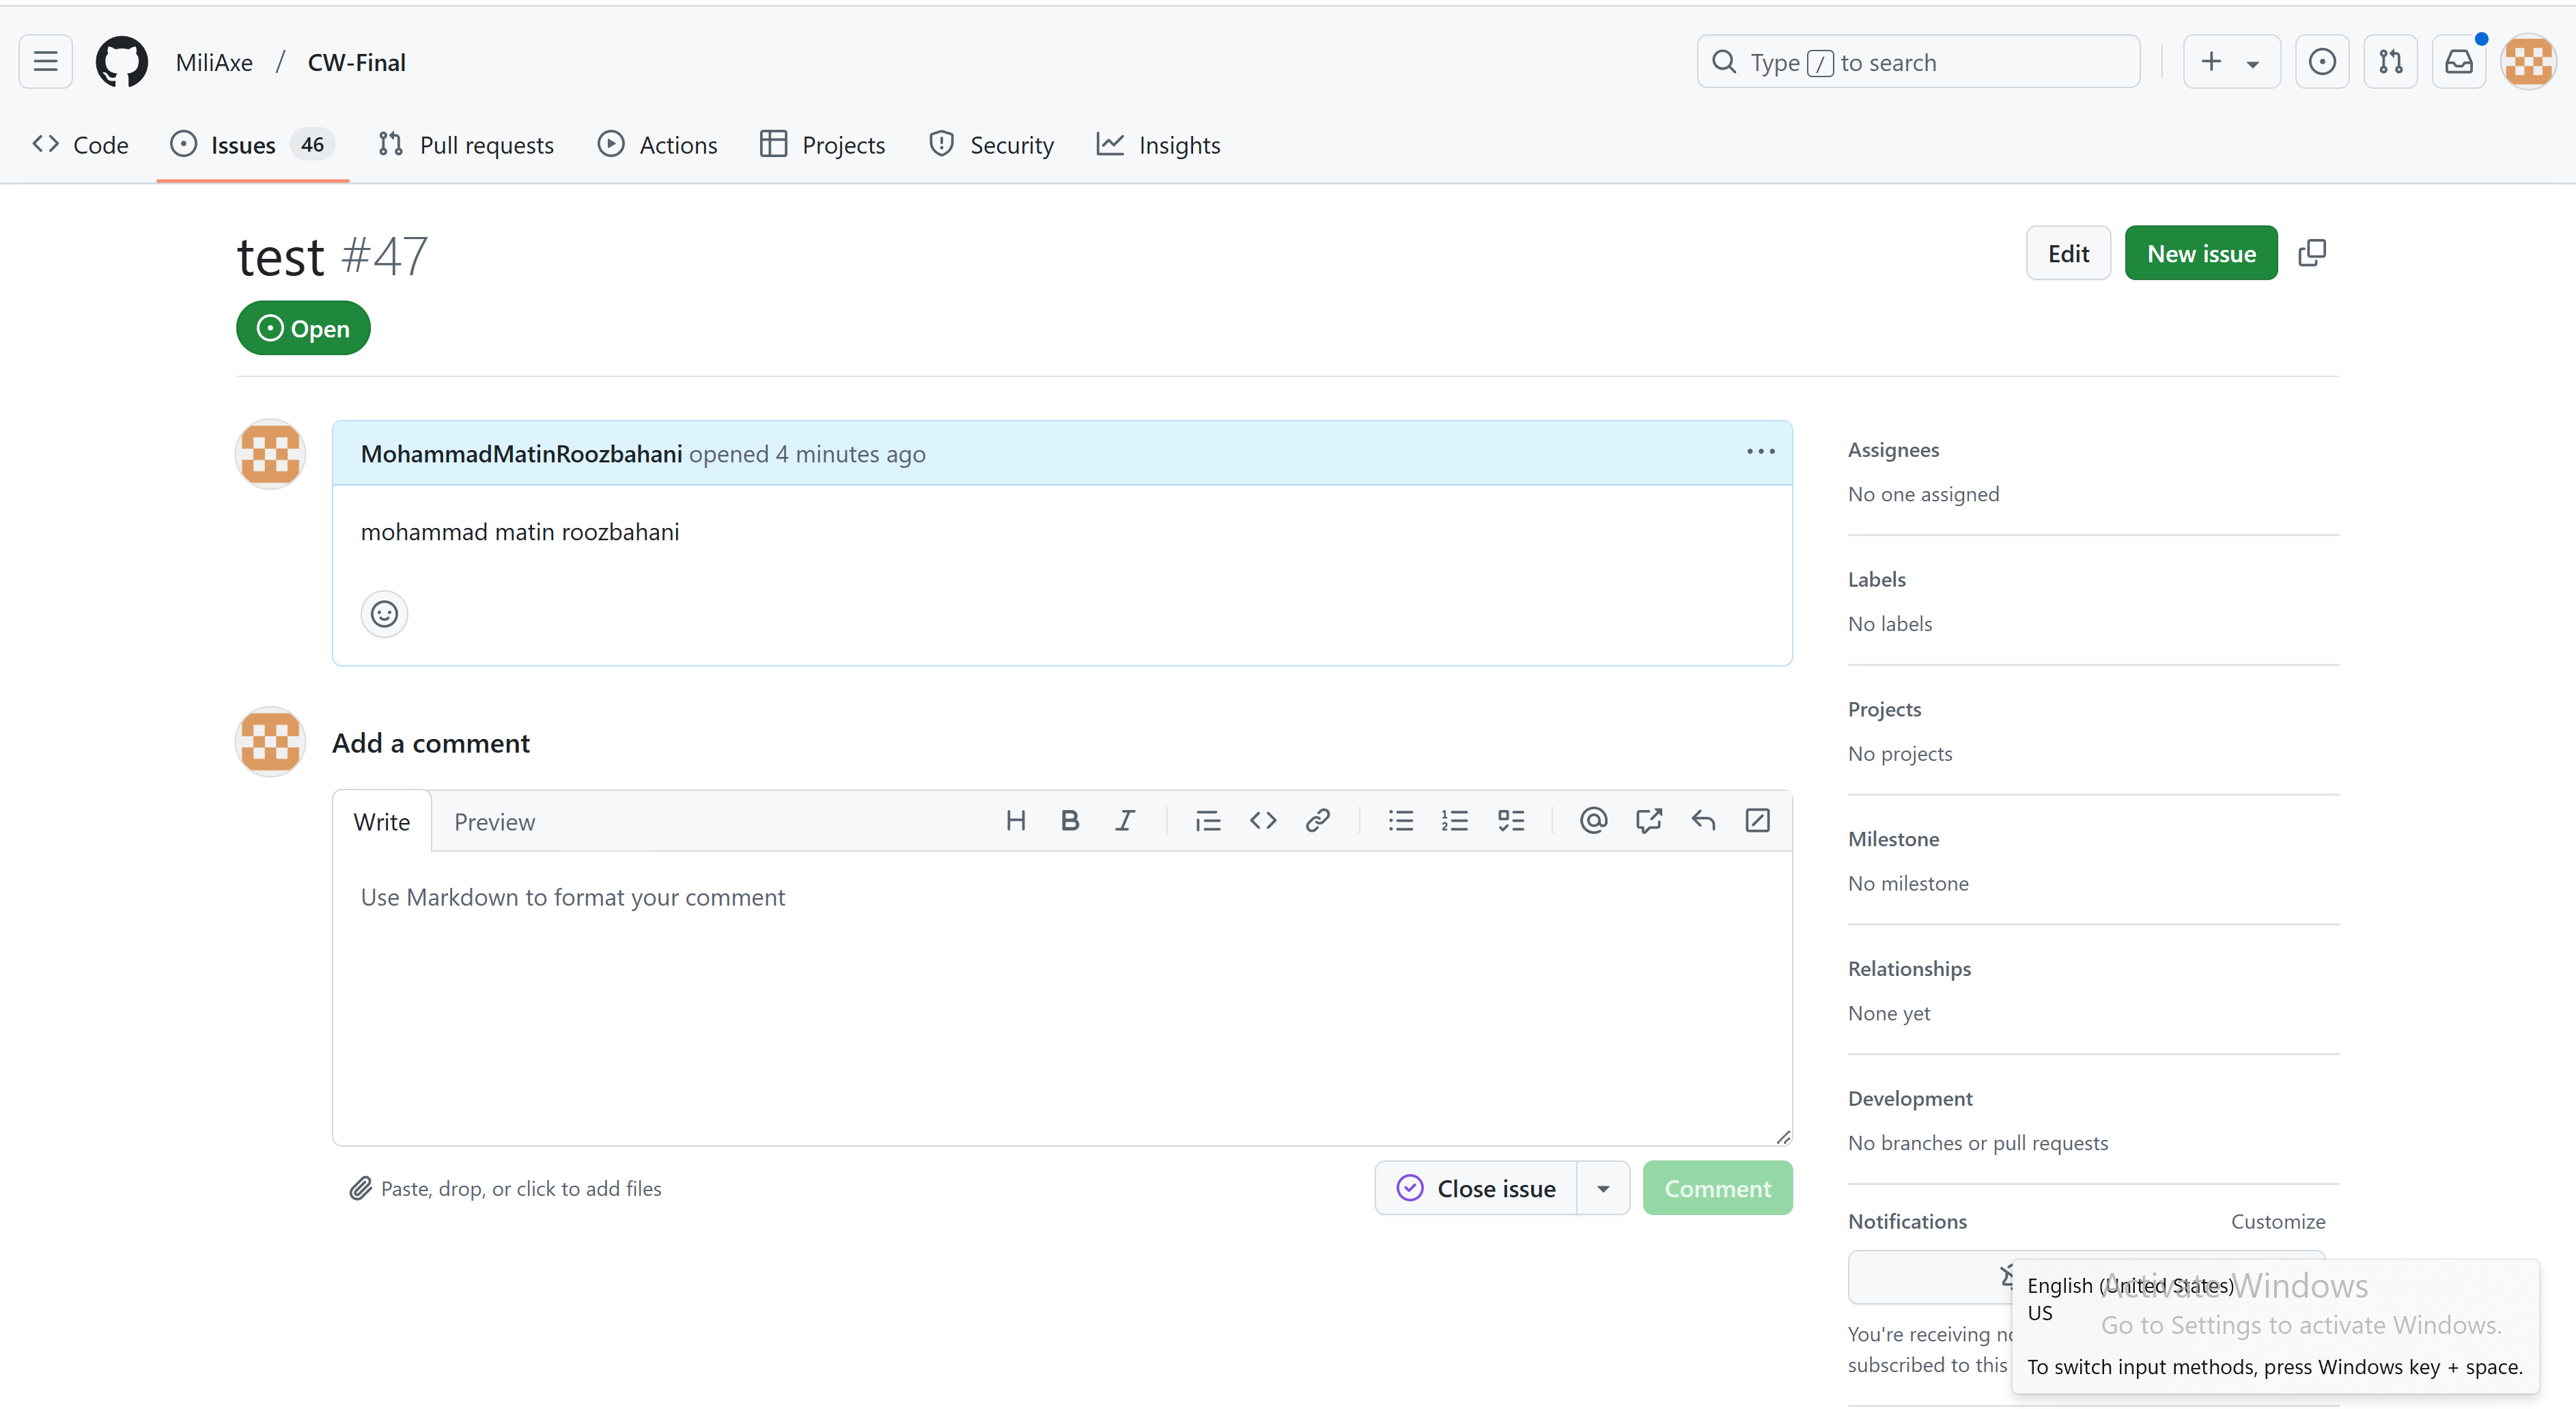
\includegraphics[width=0.7\textwidth]{mili.png}
    % اضافه کردن عنوان زیر تصویر
    % \caption{اسکرین‌شات از مشکل در GitHub}
    % تعیین برچسب برای ارجاع به تصویر
    % \label{fig:issue}
\end{figure}









\section*{3.3 FOSS Contribution}

No, because it doesn't seem interesting to me.















\end{document}